\documentclass[12pt]{article}
\usepackage{pdfpages}

\begin{document}
\title{Math in Decision Making\\ Unit on the Infinite:\\
Matching, Counting, and Comparing Large Sets}
\author{Instructor: Theron J Hitchman}
\date{Spring 2016}


\maketitle

Our main goal for the next work is to study some work of Georg Cantor on the nature of \emph{infinity}. Have you thought about that before? It turns out that infinity is a rather slippery concept. 

To make things clearer, we will have to practice speaking like mathematicians do. This will require \emph{precision}. It will also require that we build up some new language--the language of \emph{set theory}.

To keep things as ``simple'' as possible, we will mostly concern ourselves with things like counting, matching, and different types of numbers. Perhaps you have heard the terms \emph{integer}, \emph{rational number}, and \emph{real number} before? Those await you in the following pages.\\

\[
\infty
\]

\newpage
$\phantom{Theron J Hitchman}$
\newpage
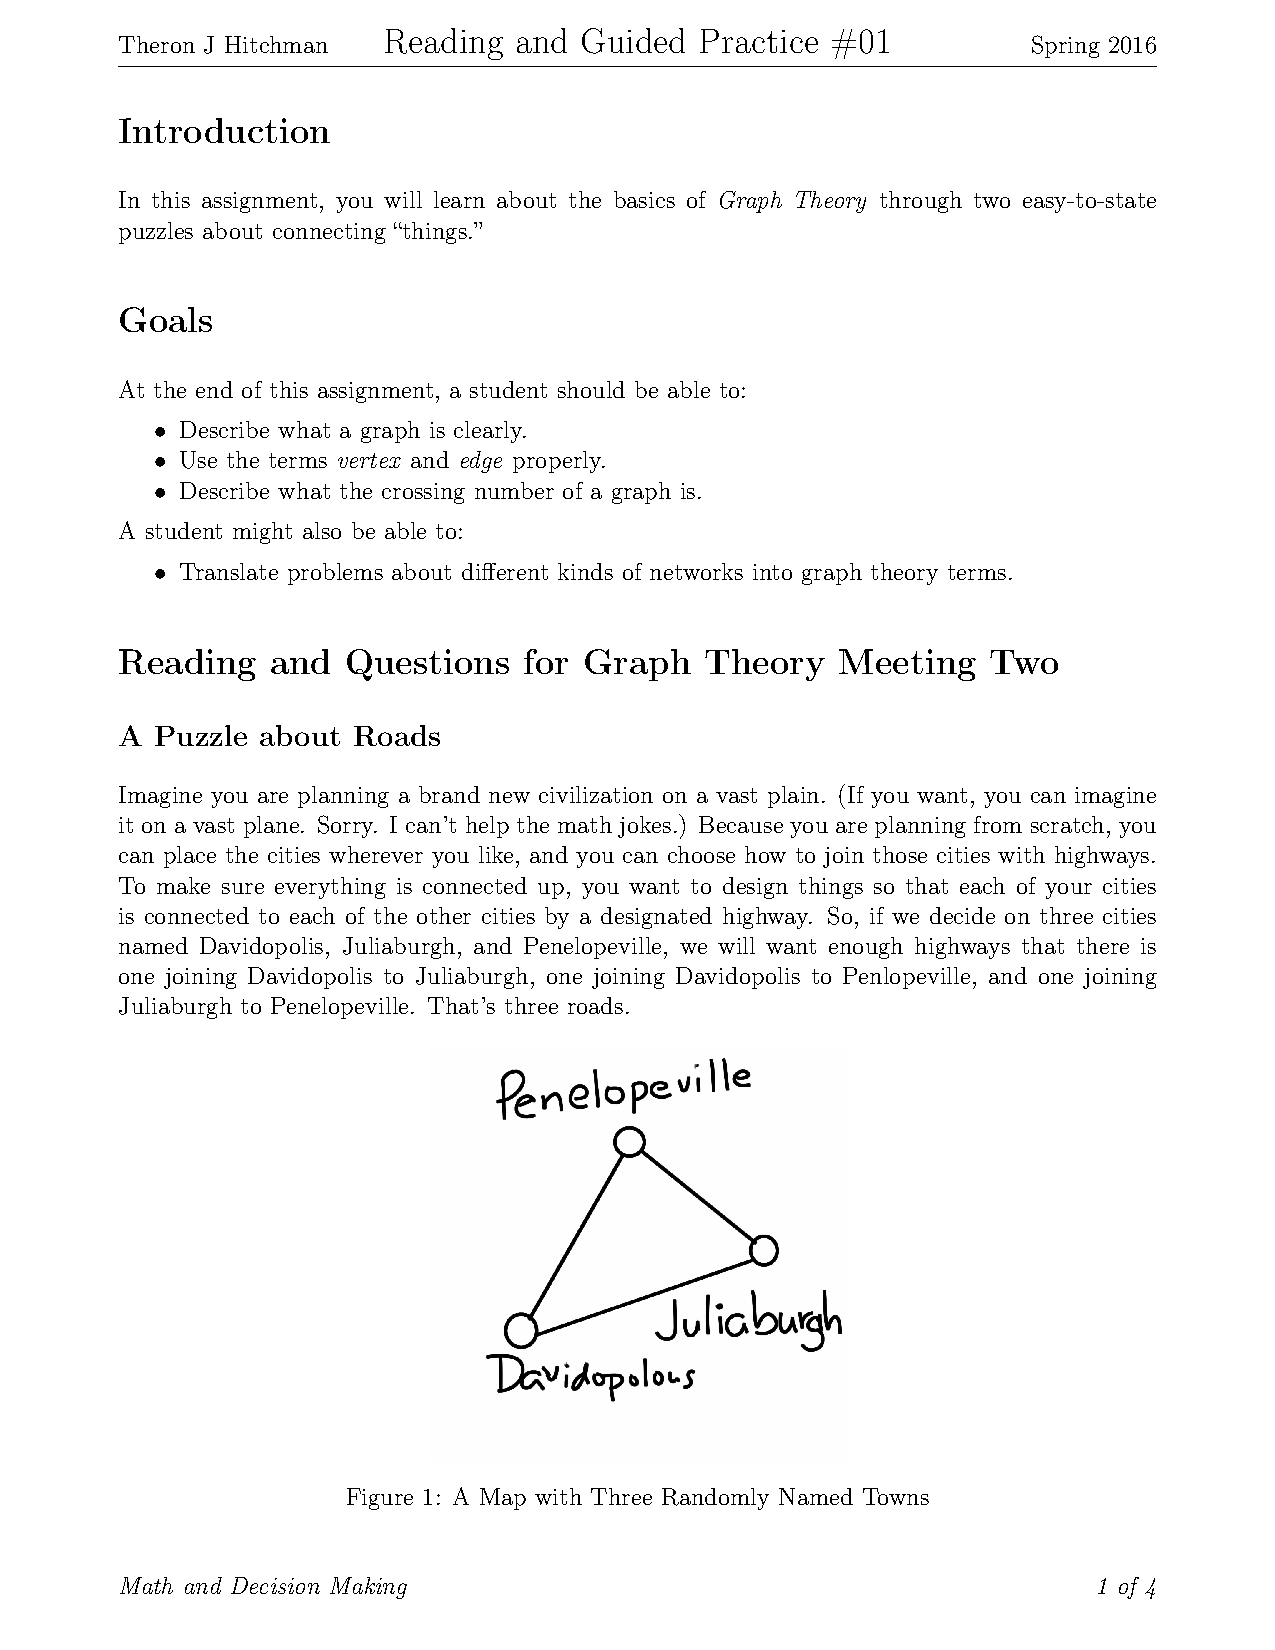
\includepdf[pages=-]{rgp01.pdf}
$\phantom{Theron J Hitchman}$
\newpage
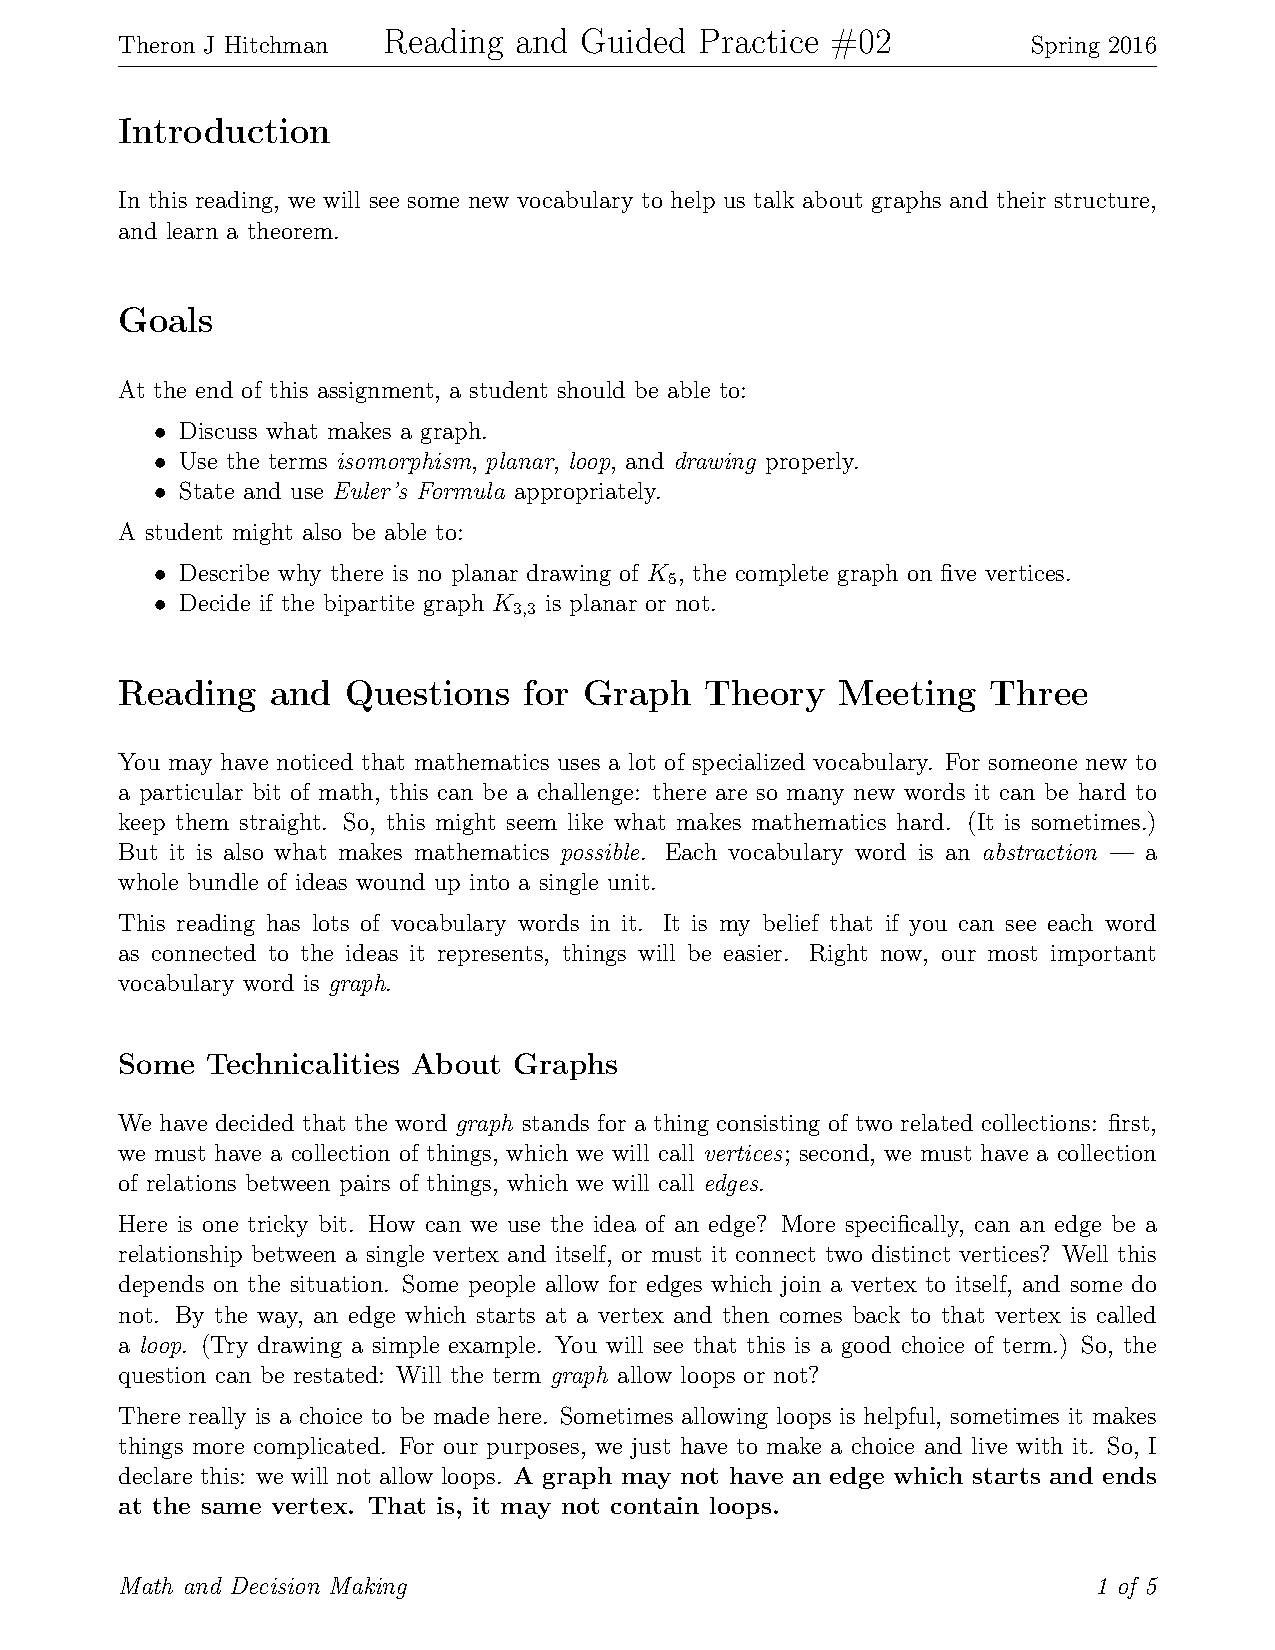
\includepdf[pages=-]{rgp02.pdf}
\newpage
$\phantom{Theron J Hitchman}$
\newpage
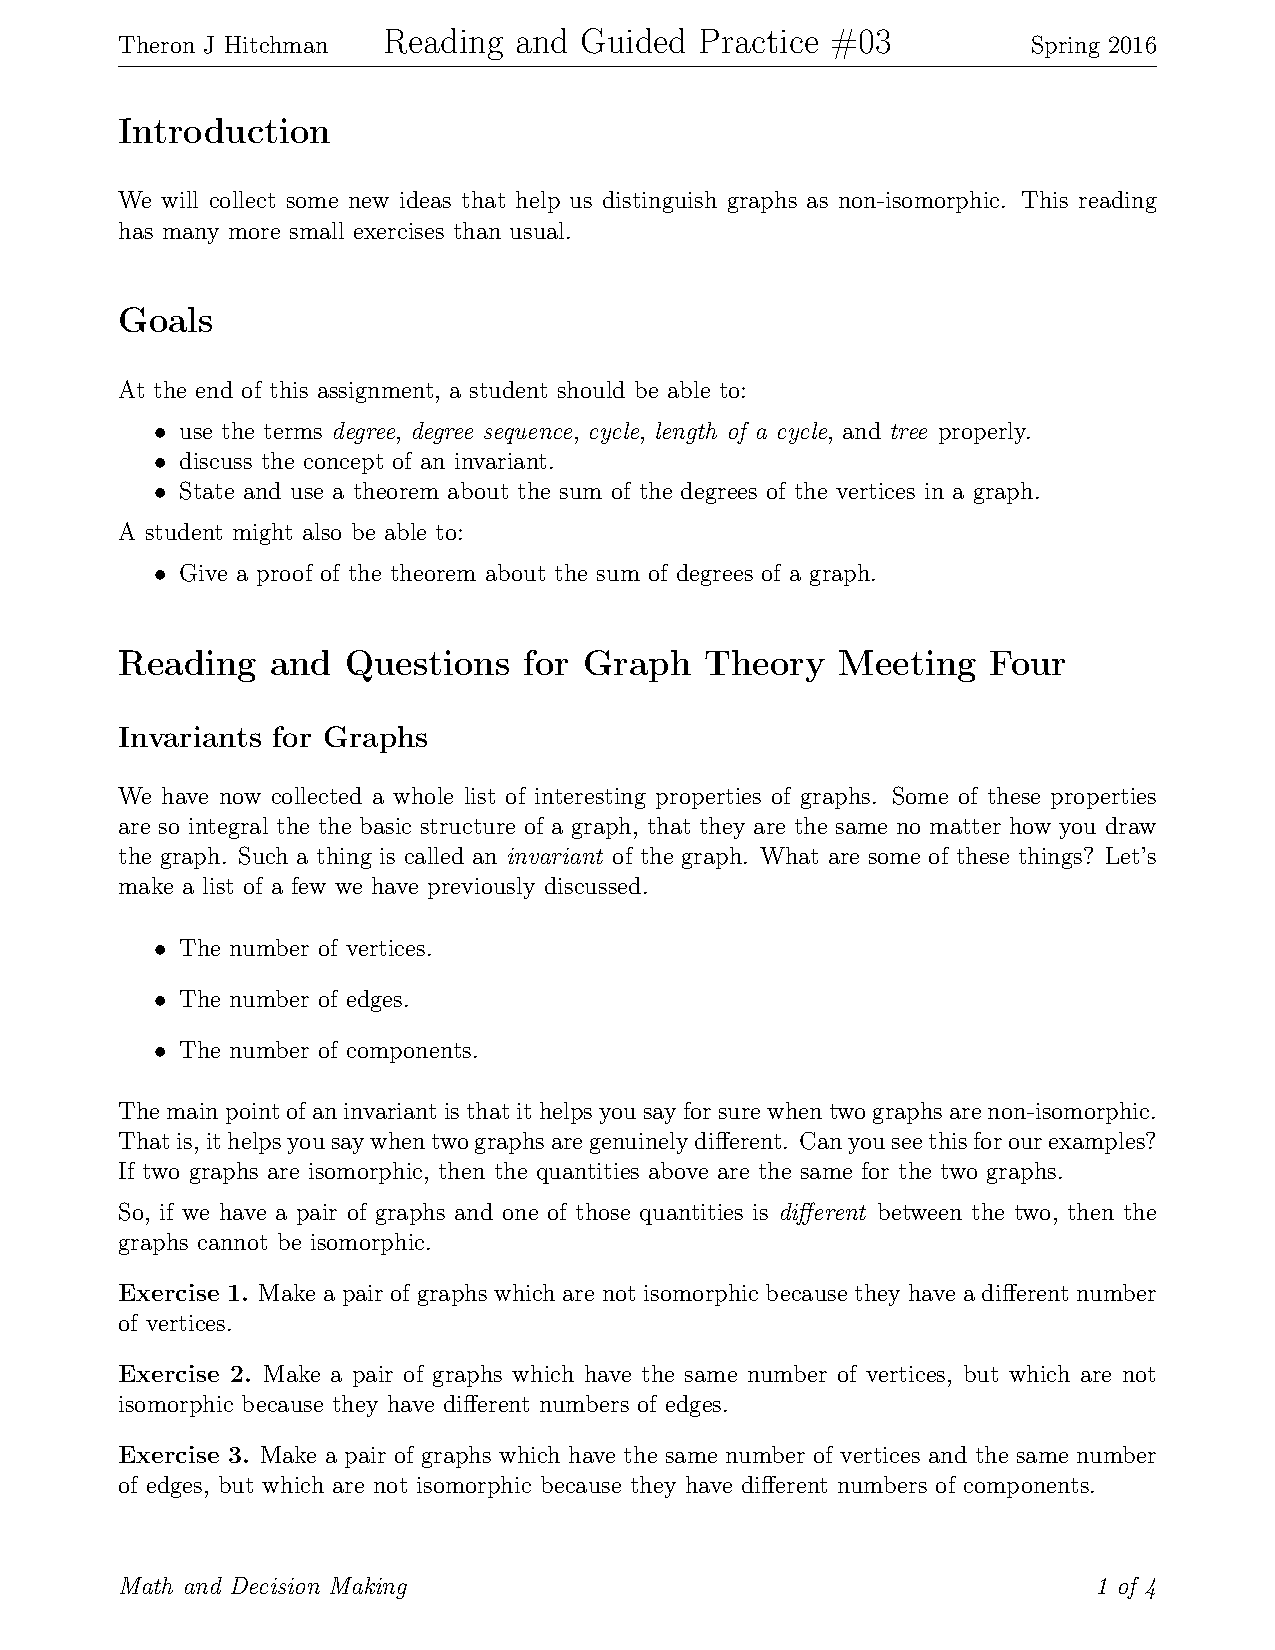
\includepdf[pages=-]{rgp03.pdf}
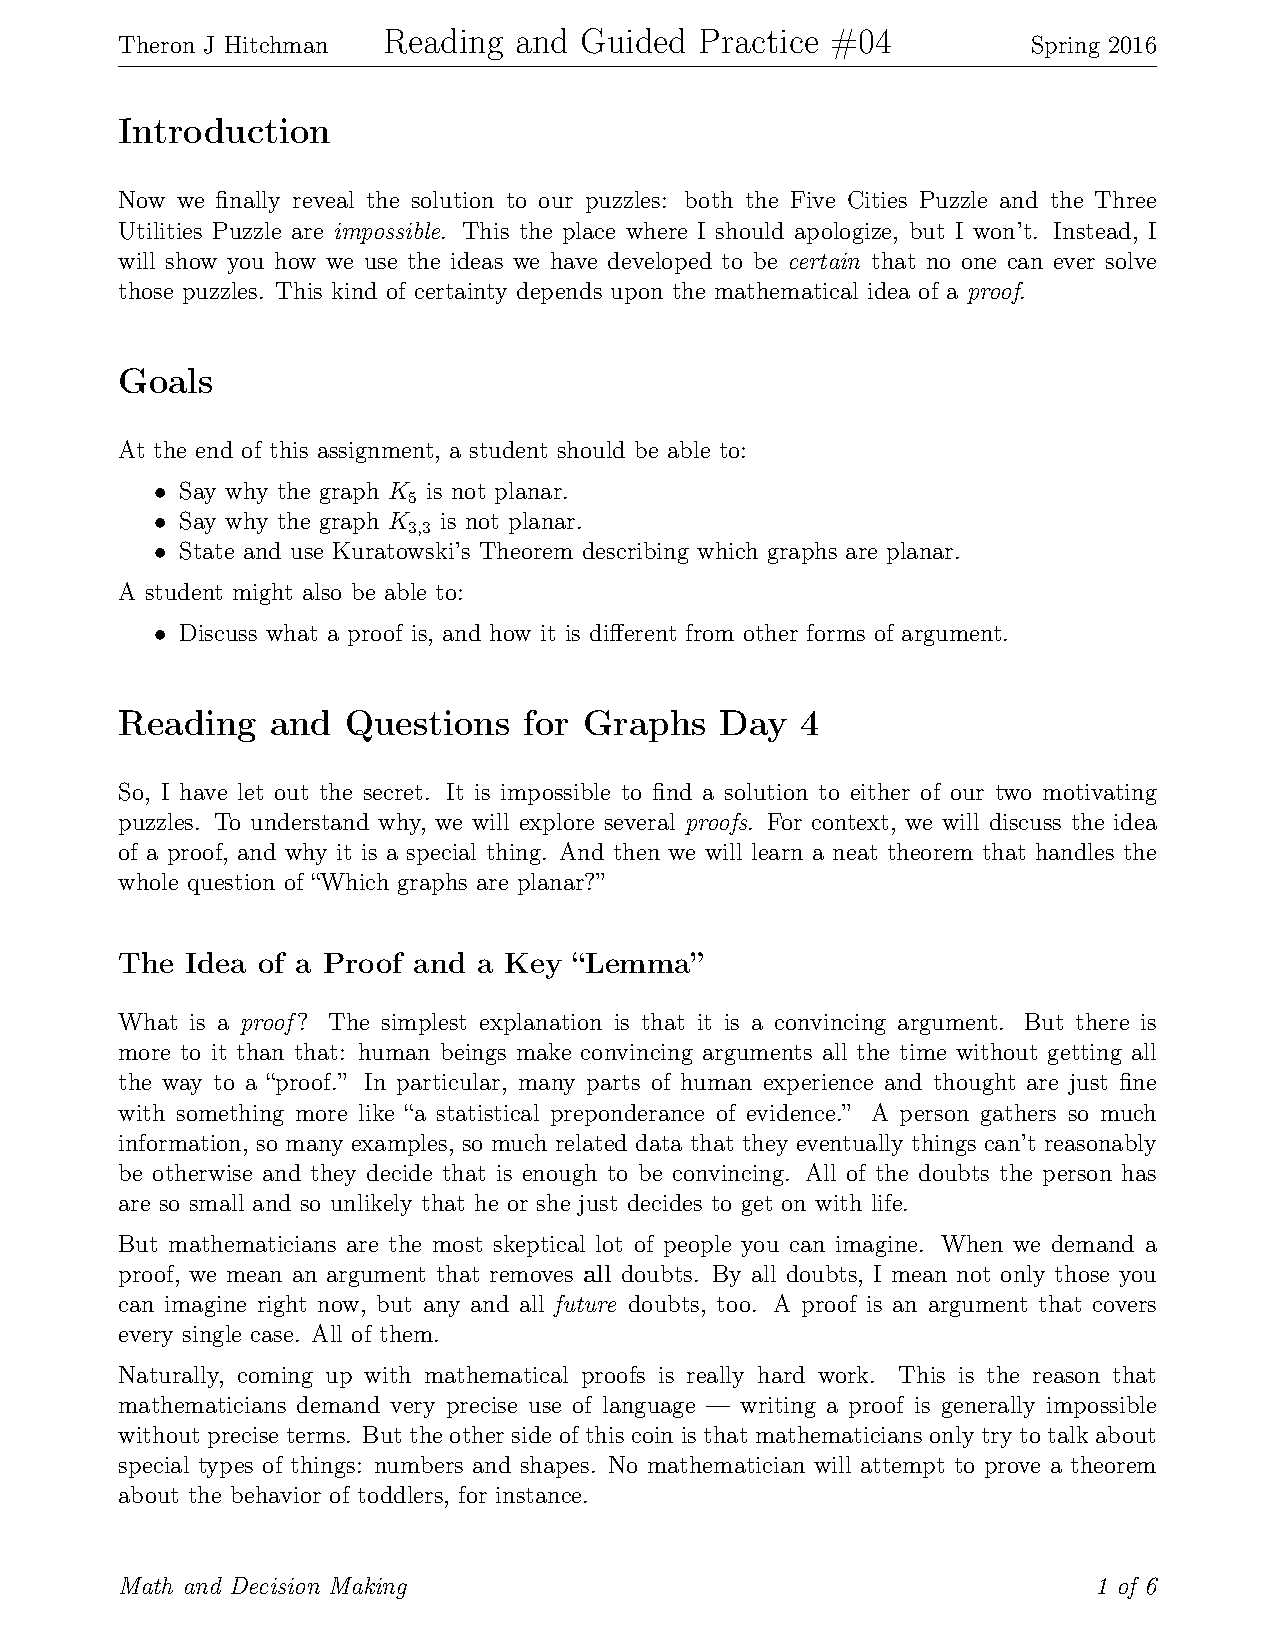
\includepdf[pages=-]{rgp04.pdf}
\newpage
$\phantom{Theron J Hitchman}$
\newpage
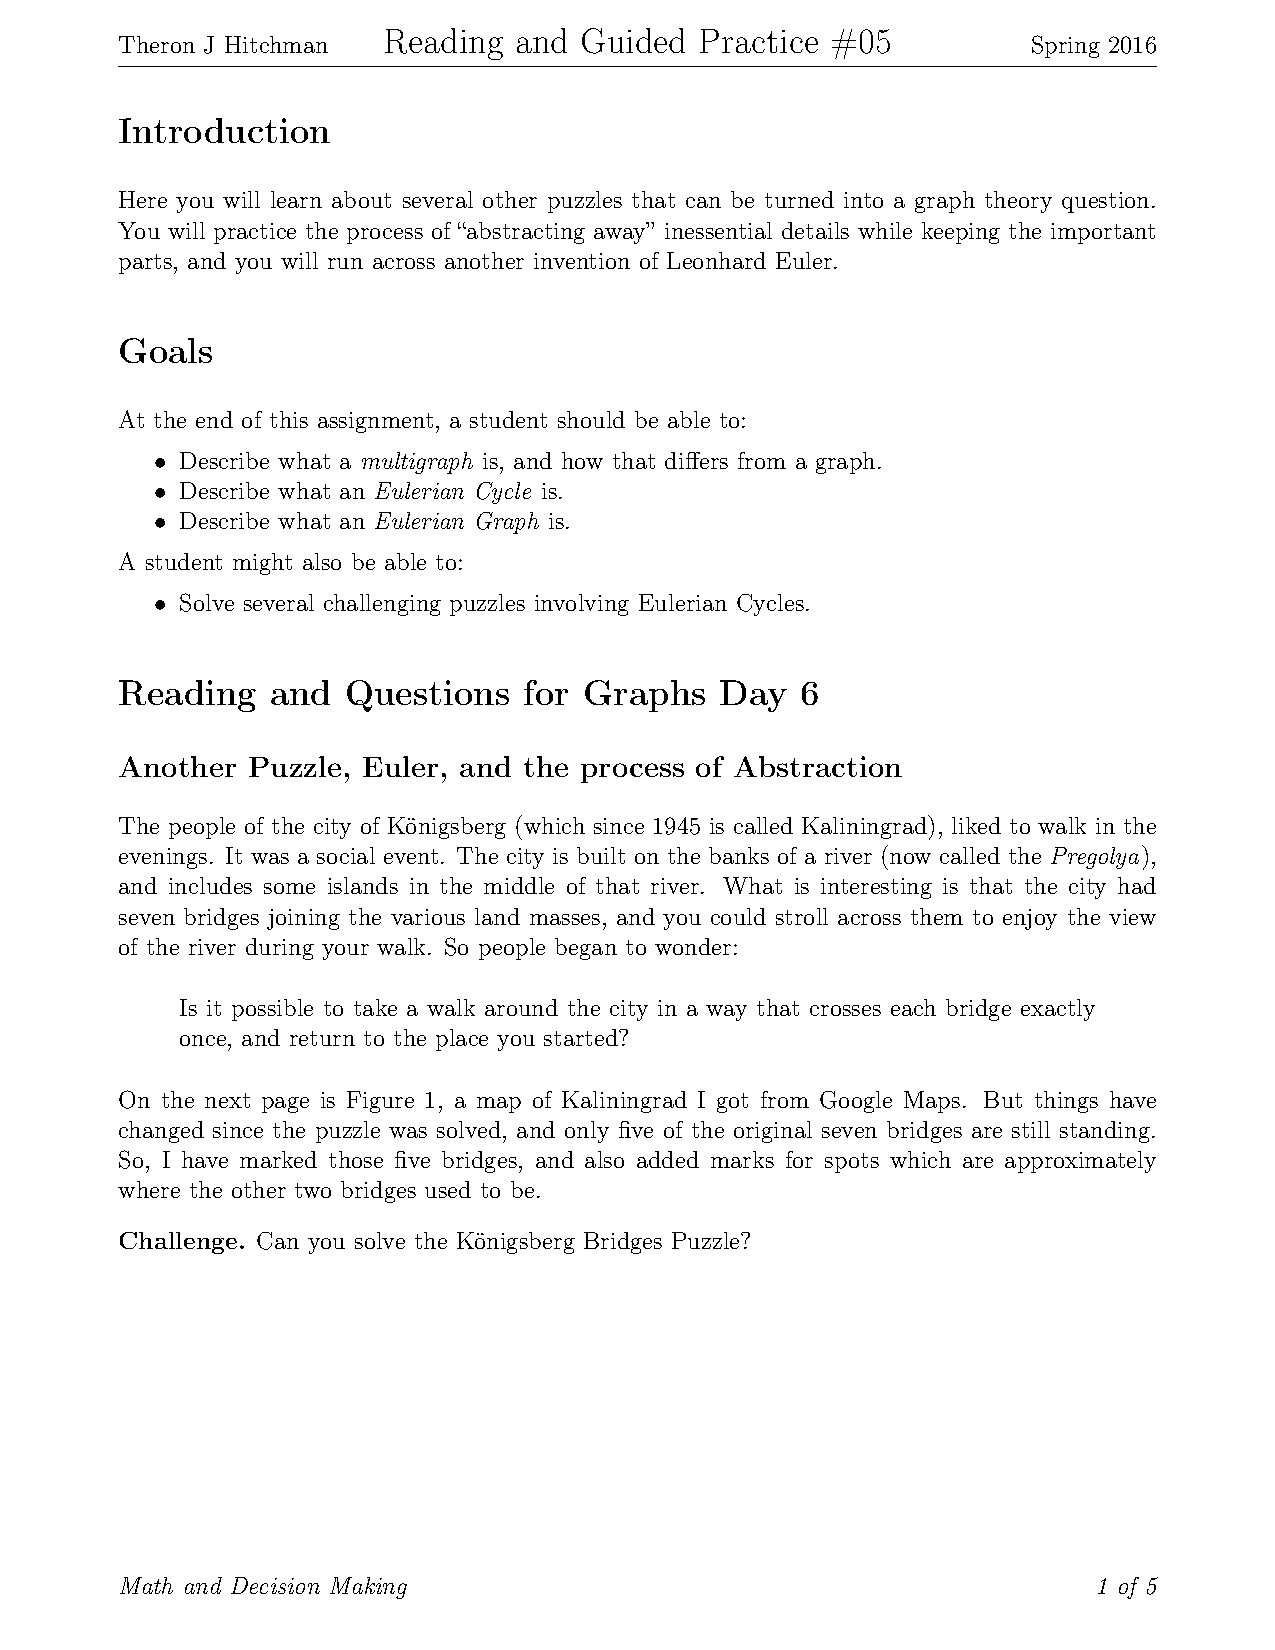
\includepdf[pages=-]{rgp05.pdf}
\newpage
$\phantom{Theron J Hitchman}$
\newpage
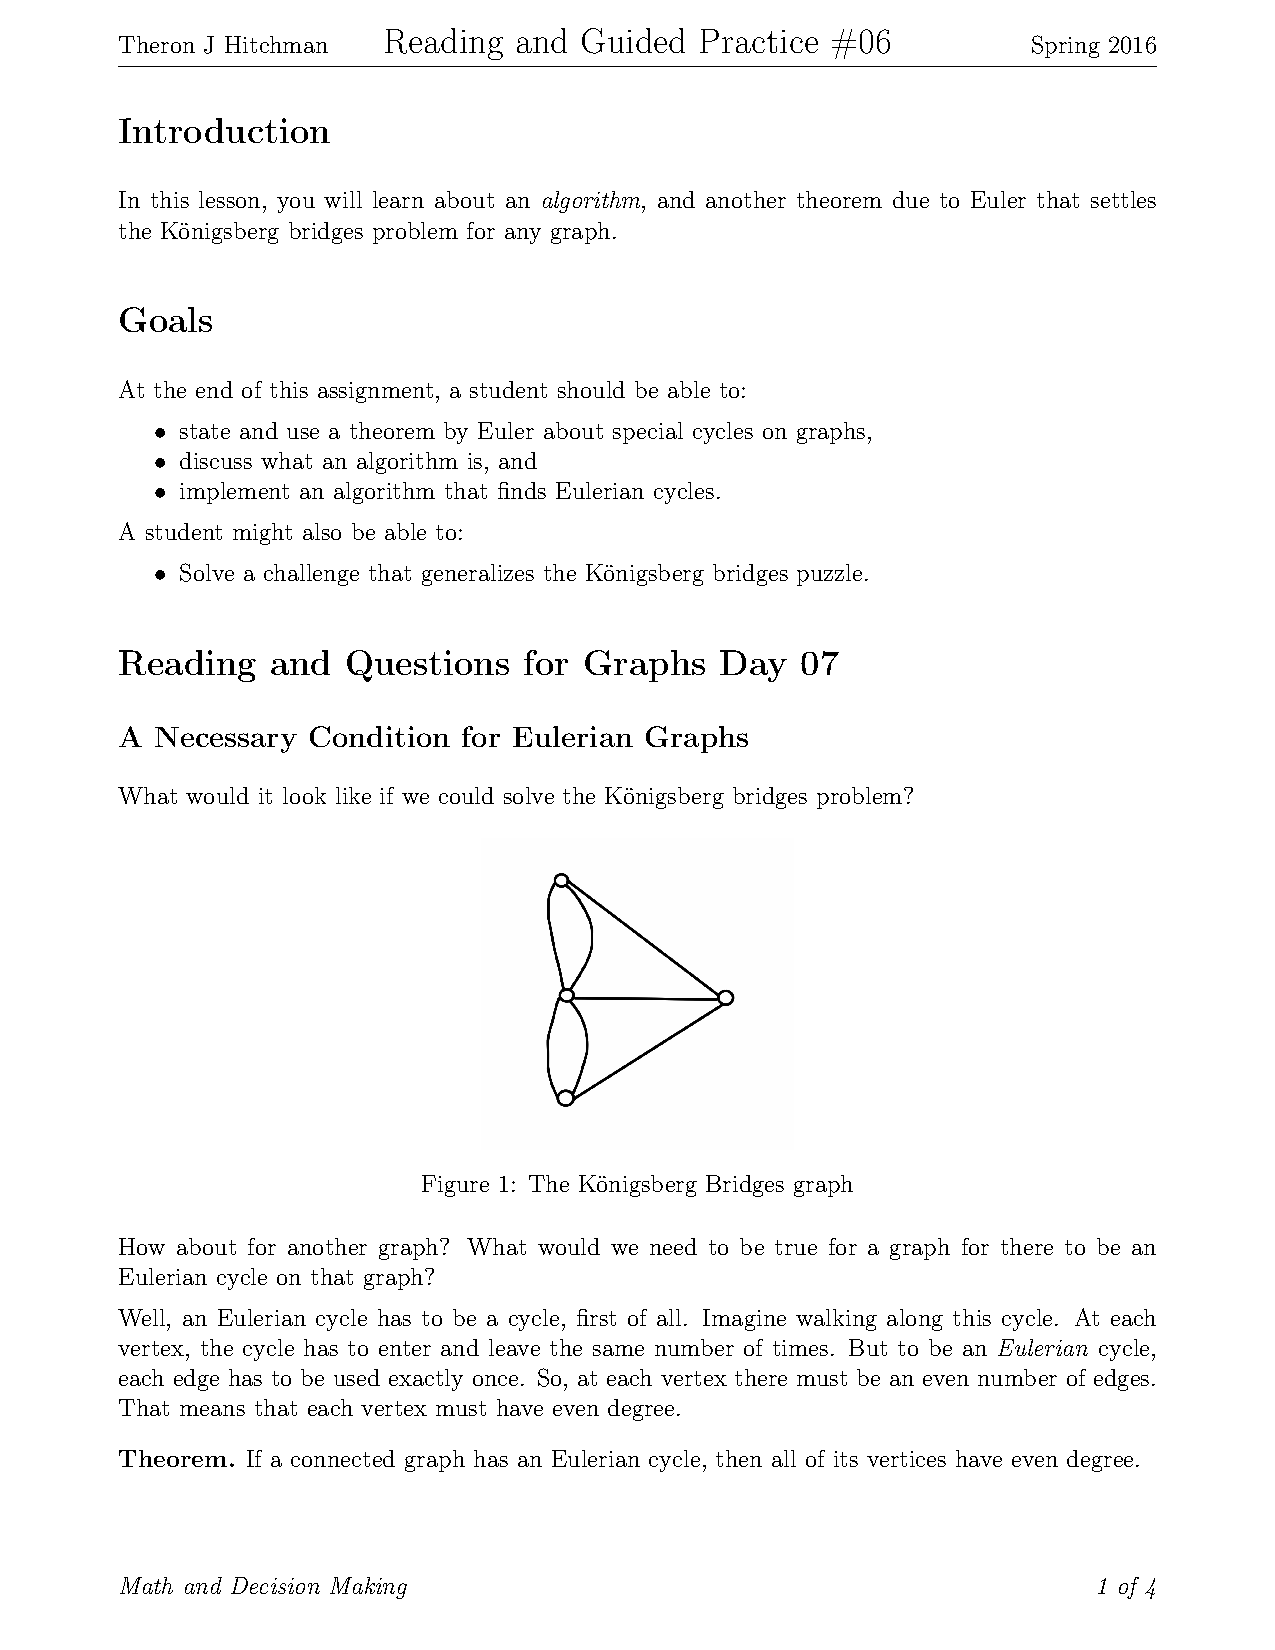
\includepdf[pages=-]{rgp06.pdf}
\newpage
$\phantom{Theron J Hitchman}$
\newpage
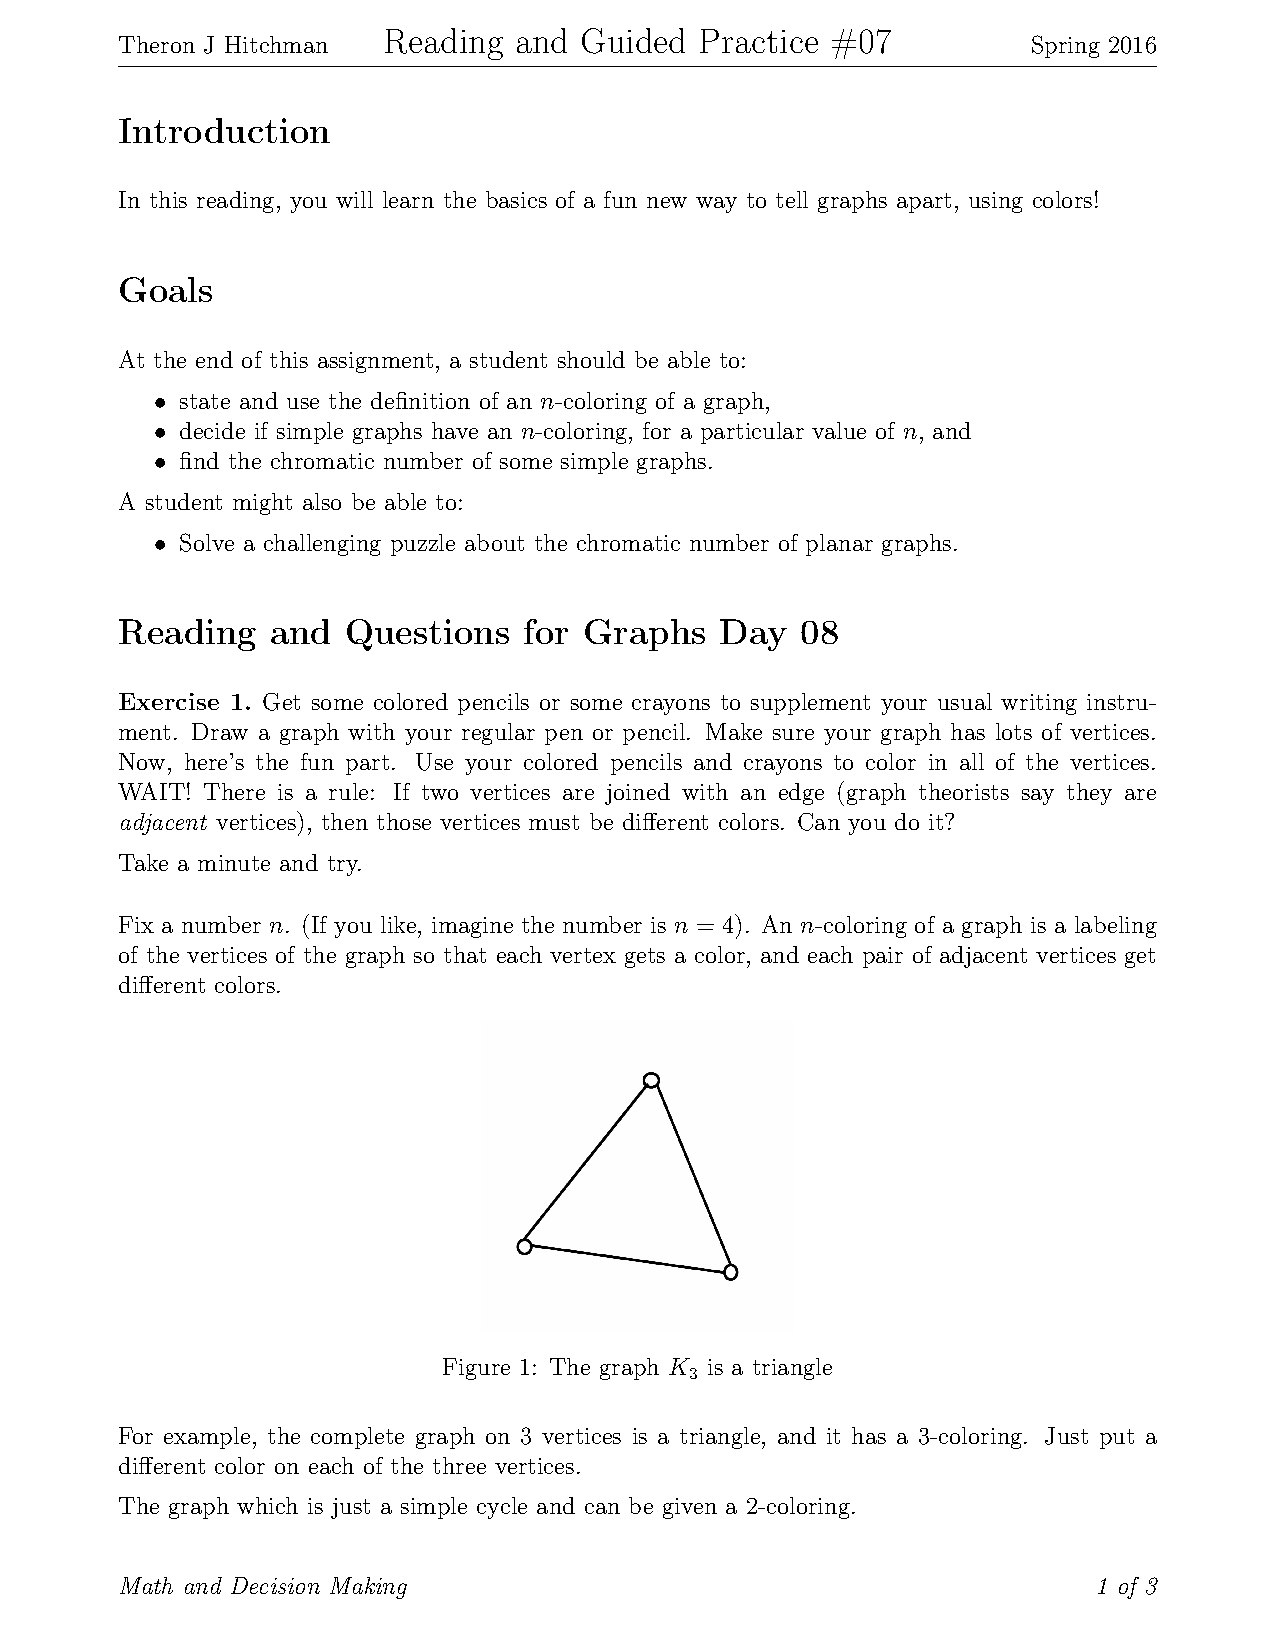
\includepdf[pages=-]{rgp07.pdf}
\newpage
$\phantom{Theron J Hitchman}$
\newpage
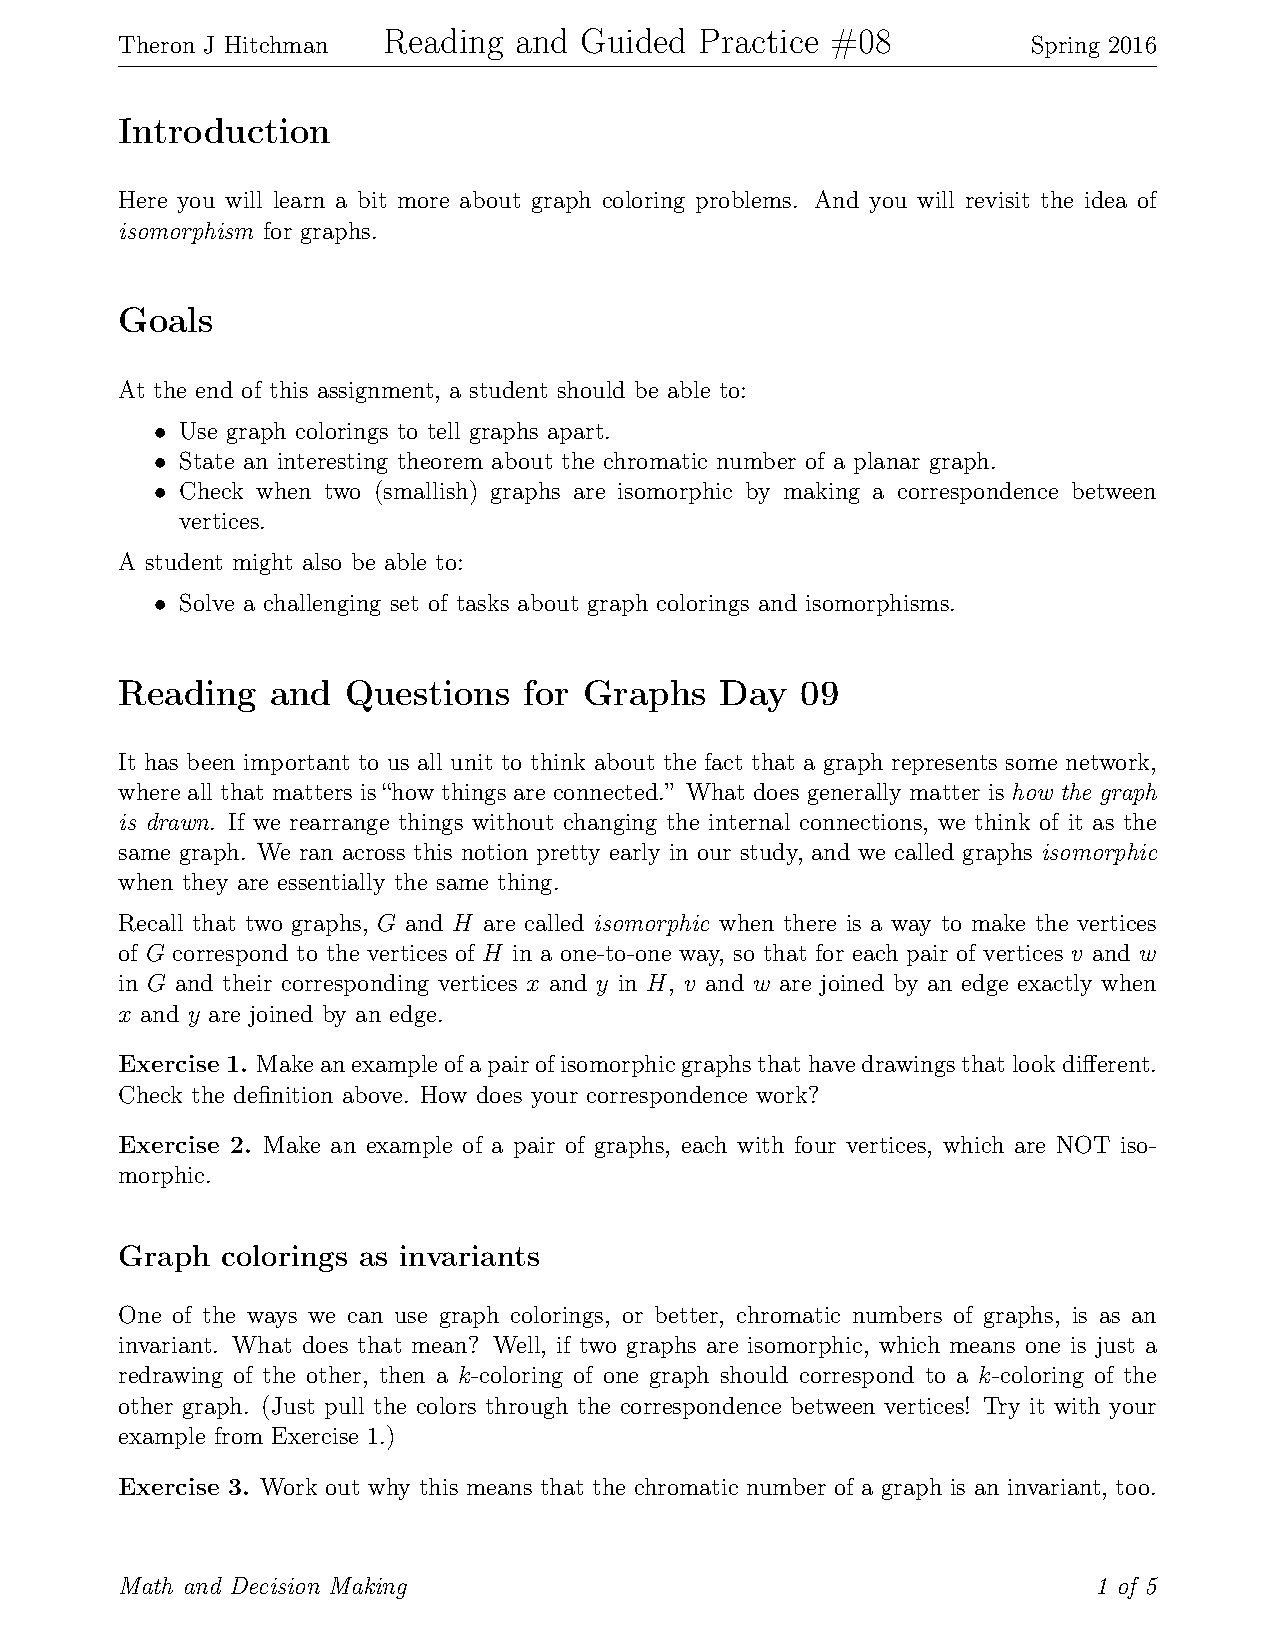
\includepdf[pages=-]{rgp08.pdf}
\newpage
$\phantom{Theron J Hitchman}$
\newpage
\includepdf[pages=-]{rgp09.pdf}
\includepdf[pages=-]{rgp10.pdf}
\includepdf[pages=-]{rgp11.pdf}
\newpage
$\phantom{Theron J Hitchman}$
\newpage
\includepdf[pages=-]{rgp12.pdf}
\includepdf[pages=-]{rgp13.pdf}

\end{document}